\documentclass[10pt,a4paper]{article}
\usepackage[utf8]{inputenc}
\usepackage{ae}
\usepackage[brazil]{babel}
\usepackage[vmargin=2cm,hmargin=2cm,columnsep=0.75cm]{geometry}
\usepackage{float,nonfloat}
\usepackage{graphicx,color}
\usepackage{subcaption}
\usepackage{amsmath}
\usepackage{verbatim}

\makeatletter
\let\@institution\empty
\def\institution#1{\def\@institution{#1}}
\renewcommand{\maketitle}{
    \begin{center}
        {\Large\bfseries\@title\par\medskip}
        {\large
            \begin{tabular}[t]{c}%
                \@author
        \end{tabular}\par\medskip}
        {\itshape\@institution\par}
        {\itshape\@date\par}
\end{center}}
\makeatother

\newcommand{\pixel}{\textit{pixel} }
\newcommand{\pixels}{\textit{pixels} }
\newcommand{\kernel}{\textit{kernel} }
\newcommand{\kernels}{\textit{kernels} }

\begin{document}
% ============================================================================

\title{MC920: Introdução ao Processamento de Imagem Digital\\Tarefa 6}
\author{
    \begin{minipage}{6cm}
        \centering
        Martin Ichilevici de Oliveira\\
        RA 118077
    \end{minipage}
    \and
    \begin{minipage}{6cm}
        \centering
        Rafael Almeida Erthal Hermano\\
        RA 121286
    \end{minipage}
}
\institution{Instituto de Computação, Universidade Estadual de Campinas}
\date{\today}

\maketitle

% ============================================================================

\section{Máscaras de Convolução e Detecção de contorno}
Detecção de contorno utiliza a primeira e segunda derivadas da imagem. A derivada de uma imagem é definida como diferenças que devem ser nulas em regiões de níveis de cinza constante, não podem ser nulas em regiões de crescimento ou decrescimento do nível de cinza.

Uma das formas mais simples de se difinir a primeira derivada em imagens digitaise dada pela fórmula:
\begin{equation}
  \frac{\partial f}{\partial x} = f(x + 1) - f(x)
  \label{eq:first_deriv}
\end{equation}

E a segunda derivada pode ser definida como:
\begin{equation}
  \frac{\partial^2 f}{\partial x^2} = f(x + 1) + f(x - 1) - 2 \cdot f(x)
  \label{eq:second_deriv}
\end{equation}

Portanto, em regiões em que a derivada é elevada, temos regiões de contorno.

\section{Gradiente e Laplaciano discretos}
\subsection{Gradiente}
O gradiente de uma imagem é uma mudança direcional na intensidade de nível de cinza de uma imagem e pode ser definido como:
\begin{equation}
  \nabla f = \frac{\partial f}{\partial x} \hat{x} + \frac{\partial f}{\partial y} \hat{y}
  \label{eq:gradient}
\end{equation}

\subsection{Laplaciano discretos}
O laplaciano de uma imagem é o operador de derivação isotrópico mais simples de uma imagem e é definido como sendo:
\begin{equation}
  \nabla^{2} f = \frac{\partial^2 f}{\partial x^2} + \frac{\partial^2 f}{\partial y^2}
  \label{eq:laplaciano}
\end{equation}

Em sua forma discreta, através da equação da segunda derivada \ref{eq:second_deriv} podemos definir o Laplaciano como:
\begin{equation}
  \nabla^{2} f = [f(x + 1, y) + f(x - 1, y) + f(x, y + 1) + f(x, y - 1)] - 4 \cdot f(x,y)
  \label{eq:discrete_laplaciano}
\end{equation}

Portanto a mascára de convolução do laplaciano é dada por:
\begin{equation}
  \nabla^{2} f =\left[\begin{array}{ccc}
    0 &  1 & 0\\
    1 & -4 & 1\\
    0 &  1 & 0
  \end{array}\right]
  \label{mask:discrete_laplaciano}
\end{equation}
\newpage

Um exemplo de aplicação do filtro pode ser observado em:
\begin{figure}[!ht]
    \centering
    \begin{subfigure}[ht]{0.45\textwidth}
        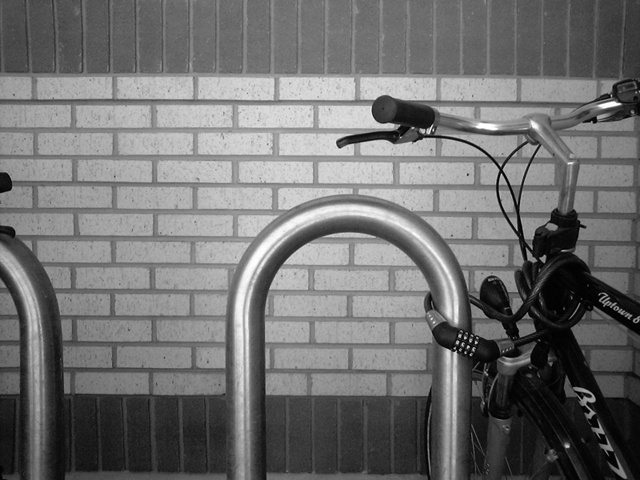
\includegraphics[width=\textwidth]{src.jpg}
        \caption{Figura original\cite{bike}}
    \end{subfigure}
    \qquad
    \begin{subfigure}[ht]{0.45\textwidth}
        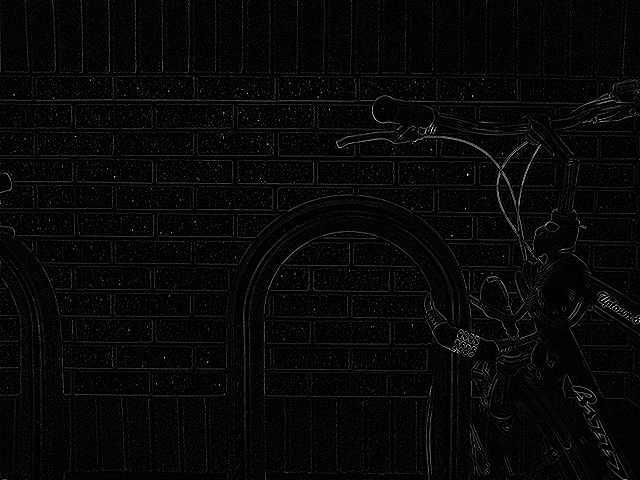
\includegraphics[width=\textwidth]{laplacian.jpg}
        \caption{\centering Após aplicação de filtro laplaciano}
    \end{subfigure}
    \label{fig:lapl}
\end{figure}

\section{Convolução e operadores direcionais}
Uma forma de calcular o gradiente, ainda que de forma, já que uma imagem digital é discrea, é através de \kernels de convolução.
\subsection{Máscaras direcionais}
\subsubsection{Sobel}
O Operador de Sobel é um operador de diferenciação discreto que calcula uma aproximação do gradiente da intensidade em cada ponto. O operador define dois \kernels, um responsáel pelo cálculo no eixo horizontal e outro pelo eixo vertical. Definimi-los:

\begin{equation}
  G_x =\left[\begin{array}{ccc}
    -1 & 0 & 1\\
    -2 & 0 & 2\\
    -1 & 0 & 1
  \end{array}\right] \qquad
  G_y =\left[\begin{array}{ccc}
    -1 & -2 & 1\\
     0 & 0 & 0\\
    1 & 2 & 1
  \end{array}\right]
  \label{eq:sobel}
\end{equation}

Para cada \pixel da imagem, calcula-se a derivada nos dois sentidos, convolucionando a imagem com os \kernels definidos em (\ref{eq:sobel}). O gradiente na imagem pode ser então aproximado combinando o resultado da operação anterior, conforme mostra (\ref{eq:sobel_combine}).

\begin{equation}
  G = \sqrt{G_x^2 + G_y^2} \qquad \text{ou} \qquad G = \frac{\left|G_x\right|+\left|G_y\right|}{2}
  \label{eq:sobel_combine}
\end{equation}

Um exemplo de aplicação do filtro pode ser observado na Figura \ref{fig:sob}.

\begin{figure}[!ht]
    \centering
    \begin{subfigure}[ht]{0.45\textwidth}
        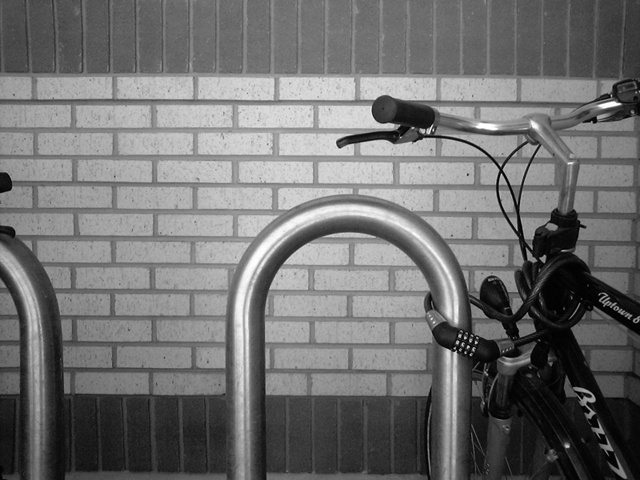
\includegraphics[width=\textwidth]{src.jpg}
        \caption{Figura original\cite{bike}}
        \label{fig:src}
    \end{subfigure}
    \qquad
    \begin{subfigure}[ht]{0.45\textwidth}
        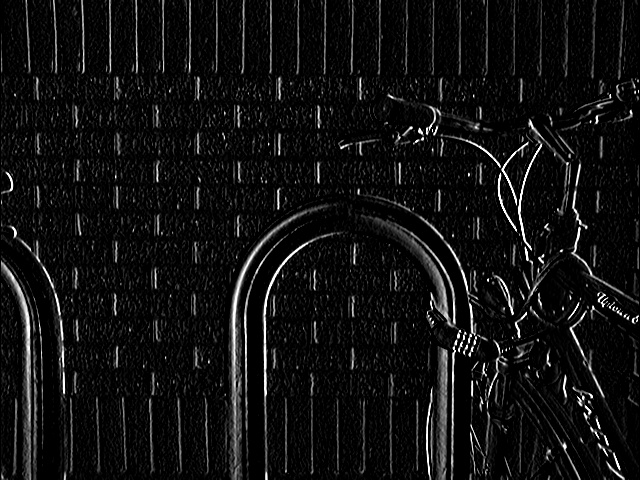
\includegraphics[width=\textwidth]{sobel_x.jpg}
        \caption{\centering Após aplicação de filtro de Sobel (com \kernel de tamanho 3) no eixo $x$}
        \label{fig:sobel_x}
    \end{subfigure}
    \\
    \begin{subfigure}[ht]{0.45\textwidth}
        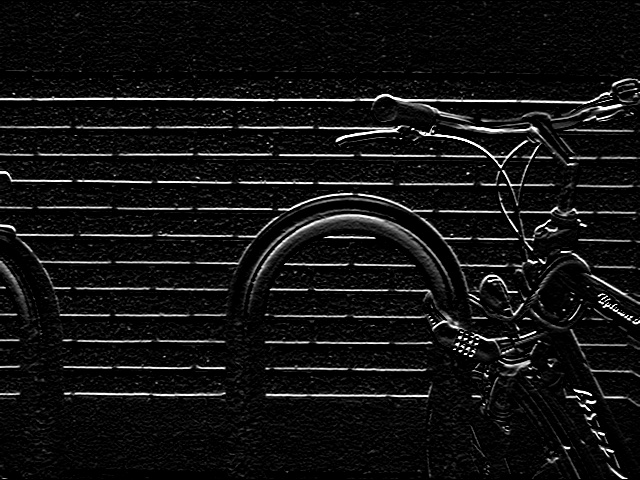
\includegraphics[width=\textwidth]{sobel_y.jpg}
        \caption{\centering Após aplicação de filtro de Sobel (com \kernel de tamanho 3) no eixo $y$}
        \label{fig:sobel_y}
    \end{subfigure}
    \qquad
    \begin{subfigure}[ht]{0.45\textwidth}
        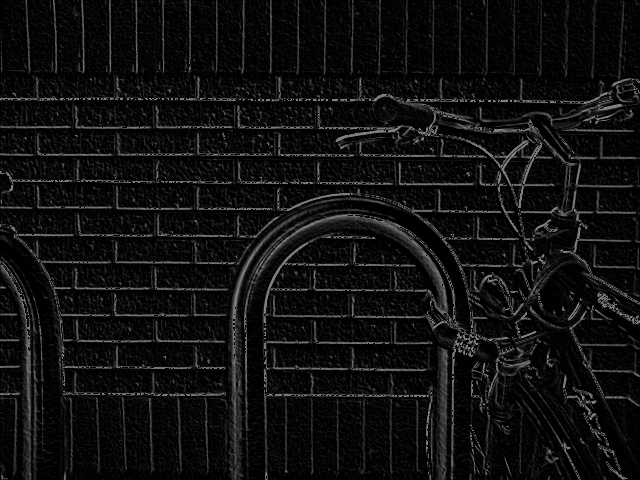
\includegraphics[width=\textwidth]{sobel.jpg}
        \caption{\centering Após aplicação de filtro de Sobel (com \kernel de tamanho 3), nos dois eixos}
        \label{fig:sobel}
    \end{subfigure}
    \caption{Imagem original e com filtro de Sobel}
    \label{fig:sob}
\end{figure}
\subsubsection{Prewitt}
O filtro de Prewitt é semelhante ao de Sobel, no sentindo de também ser formado por duas máscaras de convolução que podem ser utilizadas para detectar bordas. As máscaras são definidas por (\ref{eq:prewitt}).

\begin{equation}
  G_x =\left[\begin{array}{ccc}
    -1 & 0 & 1\\
    -1 & 0 & 1\\
    -1 & 0 & 1
  \end{array}\right] \qquad
  G_y =\left[\begin{array}{ccc}
    1 & 1 & 1\\
     0 & 0 & 0\\
    -1 & -1 & -1
  \end{array}\right]
  \label{eq:prewitt}
\end{equation}

Aplicando-se esta máscara, obtemos bons resultados, como ilustrado na Figura \ref{fig:prew}.
\begin{figure}[!ht]
    \centering
    \begin{subfigure}[ht]{0.45\textwidth}
        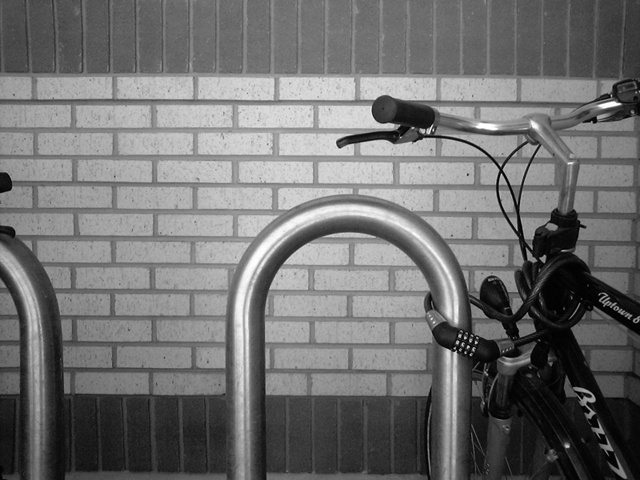
\includegraphics[width=\textwidth]{src.jpg}
        \caption{Figura original\cite{bike}}
    \end{subfigure}
    \qquad
    \begin{subfigure}[ht]{0.45\textwidth}
        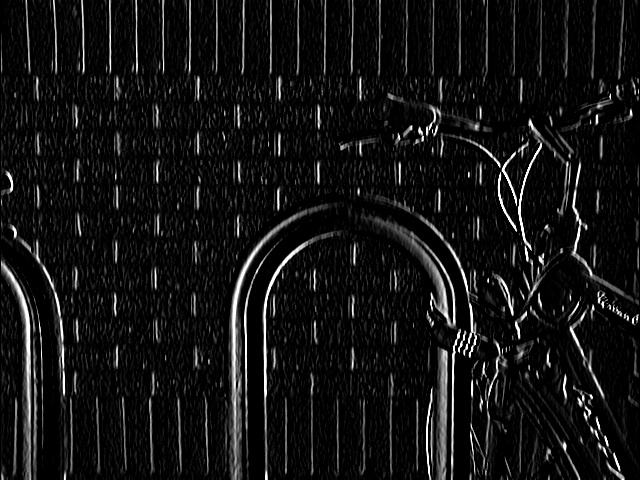
\includegraphics[width=\textwidth]{prewitt_x.jpg}
        \caption{\centering Após aplicação de filtro de Prewitt (com \kernel de tamanho 5) no eixo $x$}
        \label{fig:prewitt_x}
    \end{subfigure}
    \\
    \begin{subfigure}[ht]{0.45\textwidth}
        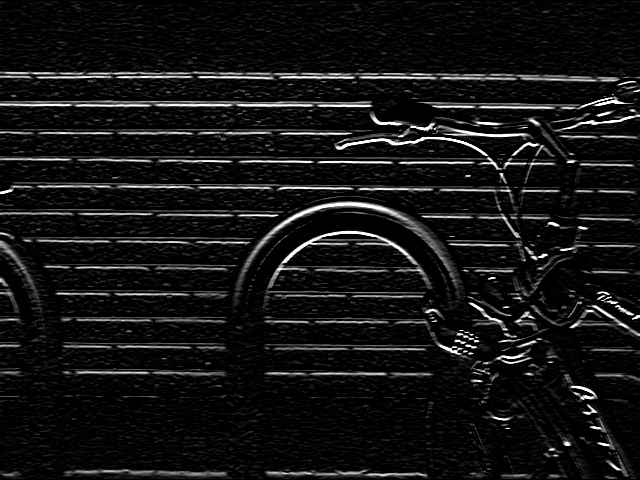
\includegraphics[width=\textwidth]{prewitt_y.jpg}
        \caption{\centering Após aplicação de filtro de Prewitt (com \kernel de tamanho 5) no eixo $y$}
        \label{fig:prewitt_y}
    \end{subfigure}
    \qquad
    \begin{subfigure}[ht]{0.45\textwidth}
        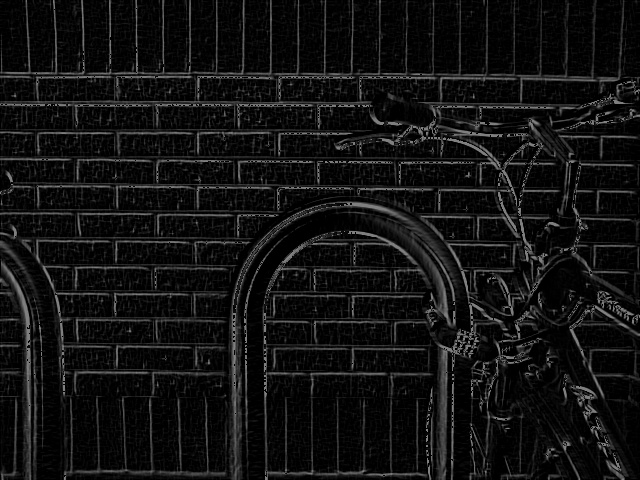
\includegraphics[width=\textwidth]{prewitt.jpg}
        \caption{\centering Após aplicação de filtro de Prewitt (com \kernel de tamanho 5), nos dois eixos}
        \label{fig:prewitt}
    \end{subfigure}
    \caption{Imagem original e com filtro de Prewitt}
    \label{fig:prew}
\end{figure}

\subsubsection{Roberts}
Outro filtro bastante utilizado na detecção de bordas é a máscara de Roberts, que pode ser expressa por (\ref{eq:roberts}). Ela tem a vantagem de ser muito rápida de calcular, já que utiliza apenas quatro \pixels. Contudo, por utilizar um \kernel tão pequeno, é mais suscetível a ruídos do que a máscara de Sobel. Um exemplo de aplicação do filtro pode ser observado na Figura \ref{fig:rob}.

\begin{equation}
  G_x =\left[\begin{array}{cc}
    1 & 0\\
    0 & -1
  \end{array}\right] \qquad
  G_y =\left[\begin{array}{cc}
    0 & 1\\
    -1 & 0
  \end{array}\right]
  \label{eq:roberts}
\end{equation}

\begin{figure}[!ht]
    \centering
    \begin{subfigure}[ht]{0.45\textwidth}
        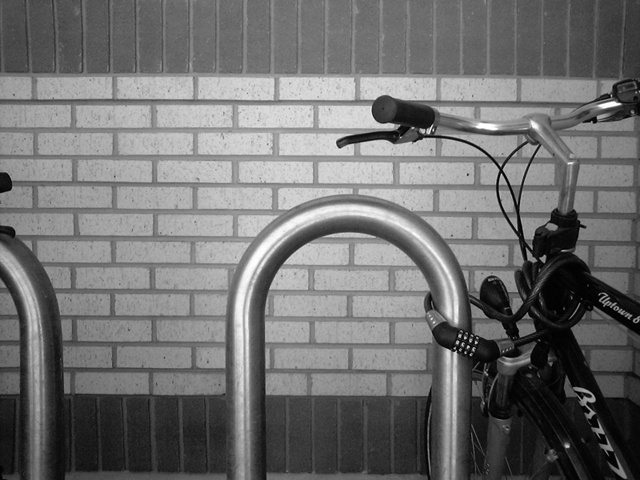
\includegraphics[width=\textwidth]{src.jpg}
        \caption{Figura original\cite{bike}}
    \end{subfigure}
    \qquad
    \begin{subfigure}[ht]{0.45\textwidth}
        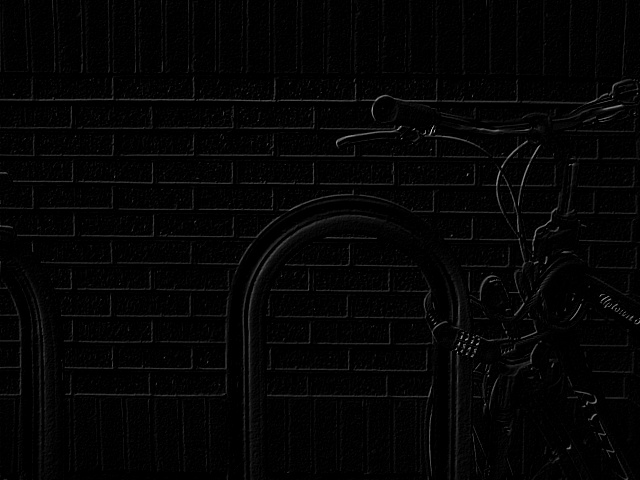
\includegraphics[width=\textwidth]{roberts_x.jpg}
        \caption{\centering Após aplicação de filtro de Roberts no eixo $x$}
        \label{fig:roberts_x}
    \end{subfigure}
    \\
    \begin{subfigure}[ht]{0.45\textwidth}
        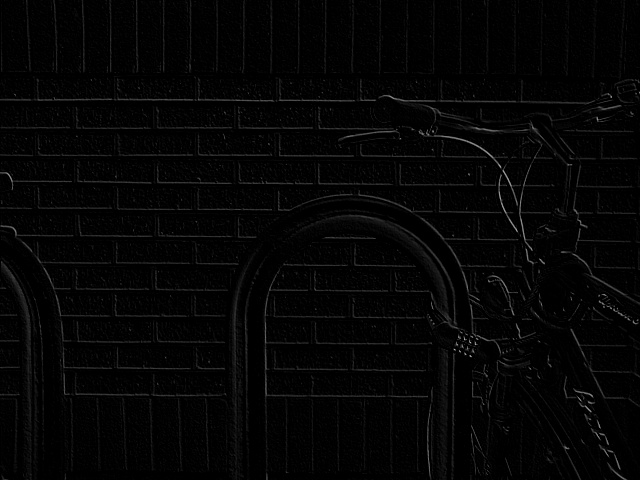
\includegraphics[width=\textwidth]{roberts_y.jpg}
        \caption{\centering Após aplicação de filtro de Roberts no eixo $y$}
        \label{fig:roberts_y}
    \end{subfigure}
    \qquad
    \begin{subfigure}[ht]{0.45\textwidth}
        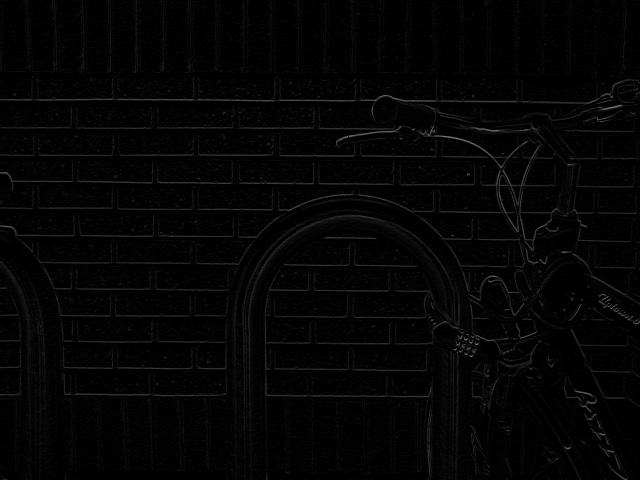
\includegraphics[width=\textwidth]{roberts.jpg}
        \caption{\centering Após aplicação de filtro de Roberts, nos dois eixos}
        \label{fig:roberts}
    \end{subfigure}
    \caption{Imagem original e com filtro de Roberts}
    \label{fig:rob}
\end{figure}

\begin{thebibliography}{99}
    \bibitem{livro} GONZALEZ, Rafael C.; WOODS, Richard E.. \textbf{Digital Image Processing}. 3. ed. Upper Saddle River, NJ, EUA: Prentice-hall, 2006.
    \bibitem{opencv-sobel} \texttt{http://docs.opencv.org/doc/tutorials/imgproc/imgtrans/sobel\_derivatives/sobel\_derivatives.html}
    \bibitem{bike} \texttt{http://en.wikipedia.org/wiki/File:Bikesgray.jpg}
\end{thebibliography}

\end{document}
